\documentclass[12pt,a4paper]{article}

\usepackage[a4paper,text={16.5cm,25.2cm},centering]{geometry}
\usepackage{lmodern}
\usepackage{amssymb,amsmath}
\usepackage{bm}
\usepackage{graphicx}
\usepackage{microtype}
\usepackage{hyperref}
\setlength{\parindent}{0pt}
\setlength{\parskip}{1.2ex}

\hypersetup
       {   pdfauthor = { Sheehan Olver },
           pdftitle={ foo },
           colorlinks=TRUE,
           linkcolor=black,
           citecolor=blue,
           urlcolor=blue
       }




\usepackage{upquote}
\usepackage{listings}
\usepackage{xcolor}
\lstset{
    basicstyle=\ttfamily\footnotesize,
    upquote=true,
    breaklines=true,
    breakindent=0pt,
    keepspaces=true,
    showspaces=false,
    columns=fullflexible,
    showtabs=false,
    showstringspaces=false,
    escapeinside={(*@}{@*)},
    extendedchars=true,
}
\newcommand{\HLJLt}[1]{#1}
\newcommand{\HLJLw}[1]{#1}
\newcommand{\HLJLe}[1]{#1}
\newcommand{\HLJLeB}[1]{#1}
\newcommand{\HLJLo}[1]{#1}
\newcommand{\HLJLk}[1]{\textcolor[RGB]{148,91,176}{\textbf{#1}}}
\newcommand{\HLJLkc}[1]{\textcolor[RGB]{59,151,46}{\textit{#1}}}
\newcommand{\HLJLkd}[1]{\textcolor[RGB]{214,102,97}{\textit{#1}}}
\newcommand{\HLJLkn}[1]{\textcolor[RGB]{148,91,176}{\textbf{#1}}}
\newcommand{\HLJLkp}[1]{\textcolor[RGB]{148,91,176}{\textbf{#1}}}
\newcommand{\HLJLkr}[1]{\textcolor[RGB]{148,91,176}{\textbf{#1}}}
\newcommand{\HLJLkt}[1]{\textcolor[RGB]{148,91,176}{\textbf{#1}}}
\newcommand{\HLJLn}[1]{#1}
\newcommand{\HLJLna}[1]{#1}
\newcommand{\HLJLnb}[1]{#1}
\newcommand{\HLJLnbp}[1]{#1}
\newcommand{\HLJLnc}[1]{#1}
\newcommand{\HLJLncB}[1]{#1}
\newcommand{\HLJLnd}[1]{\textcolor[RGB]{214,102,97}{#1}}
\newcommand{\HLJLne}[1]{#1}
\newcommand{\HLJLneB}[1]{#1}
\newcommand{\HLJLnf}[1]{\textcolor[RGB]{66,102,213}{#1}}
\newcommand{\HLJLnfm}[1]{\textcolor[RGB]{66,102,213}{#1}}
\newcommand{\HLJLnp}[1]{#1}
\newcommand{\HLJLnl}[1]{#1}
\newcommand{\HLJLnn}[1]{#1}
\newcommand{\HLJLno}[1]{#1}
\newcommand{\HLJLnt}[1]{#1}
\newcommand{\HLJLnv}[1]{#1}
\newcommand{\HLJLnvc}[1]{#1}
\newcommand{\HLJLnvg}[1]{#1}
\newcommand{\HLJLnvi}[1]{#1}
\newcommand{\HLJLnvm}[1]{#1}
\newcommand{\HLJLl}[1]{#1}
\newcommand{\HLJLld}[1]{\textcolor[RGB]{148,91,176}{\textit{#1}}}
\newcommand{\HLJLs}[1]{\textcolor[RGB]{201,61,57}{#1}}
\newcommand{\HLJLsa}[1]{\textcolor[RGB]{201,61,57}{#1}}
\newcommand{\HLJLsb}[1]{\textcolor[RGB]{201,61,57}{#1}}
\newcommand{\HLJLsc}[1]{\textcolor[RGB]{201,61,57}{#1}}
\newcommand{\HLJLsd}[1]{\textcolor[RGB]{201,61,57}{#1}}
\newcommand{\HLJLsdB}[1]{\textcolor[RGB]{201,61,57}{#1}}
\newcommand{\HLJLsdC}[1]{\textcolor[RGB]{201,61,57}{#1}}
\newcommand{\HLJLse}[1]{\textcolor[RGB]{59,151,46}{#1}}
\newcommand{\HLJLsh}[1]{\textcolor[RGB]{201,61,57}{#1}}
\newcommand{\HLJLsi}[1]{#1}
\newcommand{\HLJLso}[1]{\textcolor[RGB]{201,61,57}{#1}}
\newcommand{\HLJLsr}[1]{\textcolor[RGB]{201,61,57}{#1}}
\newcommand{\HLJLss}[1]{\textcolor[RGB]{201,61,57}{#1}}
\newcommand{\HLJLssB}[1]{\textcolor[RGB]{201,61,57}{#1}}
\newcommand{\HLJLnB}[1]{\textcolor[RGB]{59,151,46}{#1}}
\newcommand{\HLJLnbB}[1]{\textcolor[RGB]{59,151,46}{#1}}
\newcommand{\HLJLnfB}[1]{\textcolor[RGB]{59,151,46}{#1}}
\newcommand{\HLJLnh}[1]{\textcolor[RGB]{59,151,46}{#1}}
\newcommand{\HLJLni}[1]{\textcolor[RGB]{59,151,46}{#1}}
\newcommand{\HLJLnil}[1]{\textcolor[RGB]{59,151,46}{#1}}
\newcommand{\HLJLnoB}[1]{\textcolor[RGB]{59,151,46}{#1}}
\newcommand{\HLJLoB}[1]{\textcolor[RGB]{102,102,102}{\textbf{#1}}}
\newcommand{\HLJLow}[1]{\textcolor[RGB]{102,102,102}{\textbf{#1}}}
\newcommand{\HLJLp}[1]{#1}
\newcommand{\HLJLc}[1]{\textcolor[RGB]{153,153,119}{\textit{#1}}}
\newcommand{\HLJLch}[1]{\textcolor[RGB]{153,153,119}{\textit{#1}}}
\newcommand{\HLJLcm}[1]{\textcolor[RGB]{153,153,119}{\textit{#1}}}
\newcommand{\HLJLcp}[1]{\textcolor[RGB]{153,153,119}{\textit{#1}}}
\newcommand{\HLJLcpB}[1]{\textcolor[RGB]{153,153,119}{\textit{#1}}}
\newcommand{\HLJLcs}[1]{\textcolor[RGB]{153,153,119}{\textit{#1}}}
\newcommand{\HLJLcsB}[1]{\textcolor[RGB]{153,153,119}{\textit{#1}}}
\newcommand{\HLJLg}[1]{#1}
\newcommand{\HLJLgd}[1]{#1}
\newcommand{\HLJLge}[1]{#1}
\newcommand{\HLJLgeB}[1]{#1}
\newcommand{\HLJLgh}[1]{#1}
\newcommand{\HLJLgi}[1]{#1}
\newcommand{\HLJLgo}[1]{#1}
\newcommand{\HLJLgp}[1]{#1}
\newcommand{\HLJLgs}[1]{#1}
\newcommand{\HLJLgsB}[1]{#1}
\newcommand{\HLJLgt}[1]{#1}



\def\qqand{\qquad\hbox{and}\qquad}
\def\qqfor{\qquad\hbox{for}\qquad}
\def\qqas{\qquad\hbox{as}\qquad}
\def\D{ {\rm d} }
\def\I{ {\rm i} }
\def\E{ {\rm e} }
\def\C{ {\mathbb C} }
\def\R{ {\mathbb R} }
\def\CC{ {\cal C} }
\def\HH{ {\cal H} }
\def\LL{ {\cal L} }
\def\vc#1{ {\mathbf #1} }
\def\bbC{ {\mathbb C} }

\def\qqqquad{\qquad\qquad}
\def\qqwhere{\qquad\hbox{where}\qquad}
\def\Res_#1{\underset{#1}{\rm Res}\,}
\def\sech{ {\rm sech}\, }
\def\acos{ {\rm acos}\, }
\def\atan{ {\rm atan}\, }
\def\upepsilon{\varepsilon}


\def\Xint#1{ \mathchoice
   {\XXint\displaystyle\textstyle{#1} }%
   {\XXint\textstyle\scriptstyle{#1} }%
   {\XXint\scriptstyle\scriptscriptstyle{#1} }%
   {\XXint\scriptscriptstyle\scriptscriptstyle{#1} }%
   \!\int}
\def\XXint#1#2#3{ {\setbox0=\hbox{$#1{#2#3}{\int}$}
     \vcenter{\hbox{$#2#3$}}\kern-.5\wd0} }
\def\ddashint{\Xint=}
\def\dashint{\Xint-}
% \def\dashint
\def\infdashint{\dashint_{-\infty}^\infty}




\def\addtab#1={#1\;&=}
\def\ccr{\\\addtab}
\def\ip<#1>{\left\langle{#1}\right\rangle}
\def\dx{\D x}
\def\dt{\D t}
\def\dz{\D z}

\def\norm#1{\left\| #1 \right\|}

\def\pr(#1){\left({#1}\right)}
\def\br[#1]{\left[{#1}\right]}

\def\abs#1{\left|{#1}\right|}
\def\fpr(#1){\!\pr({#1})}

\def\sopmatrix#1{ \begin{pmatrix}#1\end{pmatrix} }

\def\endash{–}
\def\mdblksquare{\blacksquare}
\def\lgblksquare{\blacksquare}
\def\scre{\E}
\def\mapengine#1,#2.{\mapfunction{#1}\ifx\void#2\else\mapengine #2.\fi }

\def\map[#1]{\mapengine #1,\void.}

\def\mapenginesep_#1#2,#3.{\mapfunction{#2}\ifx\void#3\else#1\mapengine #3.\fi }

\def\mapsep_#1[#2]{\mapenginesep_{#1}#2,\void.}


\def\vcbr[#1]{\pr(#1)}


\def\bvect[#1,#2]{
{
\def\dots{\cdots}
\def\mapfunction##1{\ | \  ##1}
	\sopmatrix{
		 \,#1\map[#2]\,
	}
}
}



\def\vect[#1]{
{\def\dots{\ldots}
	\vcbr[{#1}]
} }

\def\vectt[#1]{
{\def\dots{\ldots}
	\vect[{#1}]^{\top}
} }

\def\Vectt[#1]{
{
\def\mapfunction##1{##1 \cr} 
\def\dots{\vdots}
	\begin{pmatrix}
		\map[#1]
	\end{pmatrix}
} }

\def\addtab#1={#1\;&=}
\def\ccr{\\\addtab}

\begin{document}

\textbf{M3M6: Applied Complex Analysis}

Dr. Sheehan Olver

s.olver@imperial.ac.uk

\section{Lecture 8: Matrix  functions via Cauchy's integral formula}
Here we investigate the definition of Cauchy's integral formula.

\textbf{Def (Cauchy's integral  matrix function)} Suppose $\gamma$ is a simple, closed contour that surrounds the spectrum of $A$ and $f$ is analytic in the interior. Then define

\[
f(A) := {1 \over 2 \pi \I} \oint_\gamma f(\zeta)(\zeta I - A)^{-1} \D \zeta
\]
\subsection{Equivalence to diagonalisation/Jordan canonical form}
We first show for diagonalisable $f$ this is equivalent to the definition by diagonalisation: if $A = V \Lambda V^{-1}$ we have


\begin{align*}
{1 \over 2 \pi \I} \oint_\gamma f(\zeta)(\zeta I - A)^{-1} \D \zeta &= 
{1 \over 2 \pi \I} \oint_\gamma f(\zeta) V (\zeta I - \Lambda)^{-1} V^{-1} \D \zeta \\
&= {1 \over 2 \pi \I}  V \oint_\gamma f(\zeta)  (\zeta I - \Lambda)^{-1}  \D \zeta V^{-1}\\
&=  V \sopmatrix{ {1 \over 2 \pi \I} \oint_\gamma f(\zeta)  (\zeta - \lambda_1)^{-1} \D \zeta\\
&\ddots \\ && {1 \over 2 \pi \I} \oint_\gamma f(\zeta)  (\zeta - \lambda_d)^{-1} \D \zeta }  \D \zeta V^{-1} \\
&= V \sopmatrix{ f(\lambda_1)\\
&\ddots \\ && f(\lambda_d) }  \D \zeta V^{-1}  = f(A).
\end{align*}
For Jordan canonical form we need only show its valid on Jordan blocks. Note that provided $\alpha \neq 0$ we have

\[
\sopmatrix{\alpha  & -1 \\  
            & \ddots &\ddots \\
            &&\alpha & -1 \\ &&& \alpha}^{-1} = \sopmatrix{\alpha^{-1} & \alpha^{-2} & \cdots & \alpha^{-d} \\
                                                                    & \ddots& \ddots&\vdots \\
                                                                    & & \alpha^{-1} & \alpha^{-2} \\
                                                                    &&& \alpha^{-1}}
\]
which is verifiable by inspection. Therefore for a Jordan block

\[
A =\sopmatrix{\lambda  & 1 \\  
            & \ddots &\ddots \\
            &&\lambda & 1 \\ &&& \lambda}
\]
we have


\begin{align*}
{1 \over 2 \pi \I} \oint_\gamma f(\zeta)(\zeta I - A)^{-1} \D \zeta 
&= 
{1 \over 2 \pi \I} \oint_\gamma f(\zeta) \sopmatrix{\zeta - \lambda  & -1 \\  
            & \ddots &\ddots \\
            &&\zeta - \lambda & -1 \\ &&& \zeta - \lambda}^{-1} \D \zeta \\
&= 
{1 \over 2 \pi \I} \oint_\gamma f(\zeta) \sopmatrix{(\zeta-\lambda)^{-1}\D & (\zeta-\lambda)^{-2} & \cdots & (\zeta-\lambda)^{-d} \\
                                                                    & \ddots& \ddots&  &\vdots \\
                                                                    & & (\zeta-\lambda)^{-1} & (\zeta-\lambda)^{-2} \\
                                                                    &&& (\zeta-\lambda)^{-1}} \D \zeta \\
&= \begin{pmatrix} f(\lambda) & f'(\lambda) & \cdots & f^{(d-1)}(\lambda)/(d-1)! \\
        & \ddots & \ddots & \vdots \\
            & & f(\lambda) & f'(\lambda)\\
            &&& f(\lambda)
            \end{pmatrix} = f(A).
\end{align*}
\subsection{Gershgorin circle theorem}
If we only know $A$, how do we know how big to make the contour? Gershgorin's circle theorem gives the answer:

\textbf{Theorem (Gershgorin)} Let $A \in {\mathbb C}^{d \times d}$ and define 

\[
R_k = \sum_{j=1 \atop j \neq k}^d |a_{kj}| 
\]
Then 

\[
\rho(A) \subset \bigcup_{k=1}^d \bar B(a_{kk}, R_k)
\]
where $\bar B(z_0, r)$ is the closed disk of radius $r$ and $\rho(A)$ is the set of eigenvalues.

**Proof **

We can assume any eigenvalue has at least one nonzero eigenvector, whose maximum entry is $1$ in the $k$-th entry. (Otherwise, rescale.) That is, there exists

\[
\vc v = \Vectt[v_1,\dots,v_{k-1},1,v_{k+1},\dots,v_d]
\]
so that

\[
A \vc v = \lambda \vc v
\]
The result follows from:

\[
\lambda = \vc e_k^\top (\lambda  \vc v) = \vc e_k^\top A \vc v = a_{kk} + \sum_{j \neq k} a_{kj} v_j
\]
so that

\[
|\lambda - a_{kk}| \leq \sum_{j \neq k} |a_{kj}| = R_k. 
\]
\ensuremath{\blacksquare}

\emph{Demonstration} Here we apply this to a particular matrix:


\begin{lstlisting}
(*@\HLJLk{using}@*) (*@\HLJLn{LinearAlgebra}@*)(*@\HLJLp{,}@*) (*@\HLJLn{Plots}@*)(*@\HLJLp{,}@*) (*@\HLJLn{ComplexPhasePortrait}@*)(*@\HLJLp{,}@*) (*@\HLJLn{ApproxFun}@*)
(*@\HLJLn{A}@*) (*@\HLJLoB{=}@*) (*@\HLJLp{[}@*)(*@\HLJLni{1}@*) (*@\HLJLni{2}@*) (*@\HLJLni{3}@*)(*@\HLJLp{;}@*) (*@\HLJLni{1}@*) (*@\HLJLni{5}@*) (*@\HLJLni{2}@*)(*@\HLJLp{;}@*) (*@\HLJLoB{-}@*)(*@\HLJLni{4}@*) (*@\HLJLni{1}@*) (*@\HLJLni{6}@*)(*@\HLJLp{]}@*)
\end{lstlisting}

\begin{lstlisting}
3(*@\ensuremath{\times}@*)3 Array{Int64,2}:
  1  2  3
  1  5  2
 -4  1  6
\end{lstlisting}


The following calculates the row sums:


\begin{lstlisting}
(*@\HLJLn{R}@*) (*@\HLJLoB{=}@*) (*@\HLJLnf{sum}@*)(*@\HLJLp{(}@*)(*@\HLJLn{abs}@*)(*@\HLJLoB{.}@*)(*@\HLJLp{(}@*)(*@\HLJLn{A}@*) (*@\HLJLoB{-}@*) (*@\HLJLnf{Diagonal}@*)(*@\HLJLp{(}@*)(*@\HLJLnf{diag}@*)(*@\HLJLp{(}@*)(*@\HLJLn{A}@*)(*@\HLJLp{))),}@*)(*@\HLJLn{dims}@*)(*@\HLJLoB{=}@*)(*@\HLJLni{2}@*)(*@\HLJLp{)}@*)
\end{lstlisting}

\begin{lstlisting}
3(*@\ensuremath{\times}@*)1 Array{Int64,2}:
 5
 3
 5
\end{lstlisting}


Gershgorin's theorem tells us that the spectrum lies in the union of the circles surrounding the diagonals:


\begin{lstlisting}
(*@\HLJLnf{drawcircle!}@*)(*@\HLJLp{(}@*)(*@\HLJLn{z0}@*)(*@\HLJLp{,}@*) (*@\HLJLn{R}@*)(*@\HLJLp{)}@*) (*@\HLJLoB{=}@*) (*@\HLJLnf{plot!}@*)(*@\HLJLp{(}@*)(*@\HLJLn{\ensuremath{\theta}}@*)(*@\HLJLoB{->}@*) (*@\HLJLnf{real}@*)(*@\HLJLp{(}@*)(*@\HLJLn{z0}@*)(*@\HLJLp{)}@*) (*@\HLJLoB{+}@*) (*@\HLJLn{R}@*)(*@\HLJLp{[}@*)(*@\HLJLni{1}@*)(*@\HLJLp{]}@*)(*@\HLJLoB{*}@*)(*@\HLJLnf{cos}@*)(*@\HLJLp{(}@*)(*@\HLJLn{\ensuremath{\theta}}@*)(*@\HLJLp{),}@*) (*@\HLJLn{\ensuremath{\theta}}@*)(*@\HLJLoB{->}@*) (*@\HLJLnf{imag}@*)(*@\HLJLp{(}@*)(*@\HLJLn{z0}@*)(*@\HLJLp{)}@*) (*@\HLJLoB{+}@*) (*@\HLJLn{R}@*)(*@\HLJLp{[}@*)(*@\HLJLni{1}@*)(*@\HLJLp{]}@*)(*@\HLJLoB{*}@*)(*@\HLJLnf{sin}@*)(*@\HLJLp{(}@*)(*@\HLJLn{\ensuremath{\theta}}@*)(*@\HLJLp{),}@*) (*@\HLJLni{0}@*)(*@\HLJLp{,}@*) (*@\HLJLni{2}@*)(*@\HLJLn{\ensuremath{\pi}}@*)(*@\HLJLp{,}@*) (*@\HLJLn{fill}@*)(*@\HLJLoB{=}@*)(*@\HLJLp{(}@*)(*@\HLJLni{0}@*)(*@\HLJLp{,}@*)(*@\HLJLoB{:}@*)(*@\HLJLn{red}@*)(*@\HLJLp{),}@*) (*@\HLJLn{\ensuremath{\alpha}}@*) (*@\HLJLoB{=}@*) (*@\HLJLnfB{0.2}@*)(*@\HLJLp{,}@*) (*@\HLJLn{legend}@*)(*@\HLJLoB{=}@*)(*@\HLJLkc{false}@*)(*@\HLJLp{)}@*)

(*@\HLJLn{\ensuremath{\lambda}}@*) (*@\HLJLoB{=}@*) (*@\HLJLnf{eigvals}@*)(*@\HLJLp{(}@*)(*@\HLJLn{A}@*)(*@\HLJLp{)}@*)
(*@\HLJLn{p}@*) (*@\HLJLoB{=}@*) (*@\HLJLnf{plot}@*)(*@\HLJLp{()}@*)
(*@\HLJLk{for}@*) (*@\HLJLn{k}@*) (*@\HLJLoB{=}@*) (*@\HLJLni{1}@*)(*@\HLJLoB{:}@*)(*@\HLJLnf{size}@*)(*@\HLJLp{(}@*)(*@\HLJLn{A}@*)(*@\HLJLp{,}@*)(*@\HLJLni{1}@*)(*@\HLJLp{)}@*)
    (*@\HLJLnf{drawcircle!}@*)(*@\HLJLp{(}@*)(*@\HLJLn{A}@*)(*@\HLJLp{[}@*)(*@\HLJLn{k}@*)(*@\HLJLp{,}@*)(*@\HLJLn{k}@*)(*@\HLJLp{],}@*) (*@\HLJLn{R}@*)(*@\HLJLp{[}@*)(*@\HLJLn{k}@*)(*@\HLJLp{])}@*)
(*@\HLJLk{end}@*)
(*@\HLJLnf{scatter!}@*)(*@\HLJLp{(}@*)(*@\HLJLn{complex}@*)(*@\HLJLoB{.}@*)(*@\HLJLp{(}@*)(*@\HLJLn{\ensuremath{\lambda}}@*)(*@\HLJLp{);}@*) (*@\HLJLn{label}@*)(*@\HLJLoB{=}@*)(*@\HLJLs{"{}eigenvalues"{}}@*)(*@\HLJLp{)}@*)
(*@\HLJLnf{scatter!}@*)(*@\HLJLp{(}@*)(*@\HLJLn{complex}@*)(*@\HLJLoB{.}@*)(*@\HLJLp{(}@*)(*@\HLJLnf{diag}@*)(*@\HLJLp{(}@*)(*@\HLJLn{A}@*)(*@\HLJLp{));}@*) (*@\HLJLn{label}@*)(*@\HLJLoB{=}@*)(*@\HLJLs{"{}diagonals"{}}@*)(*@\HLJLp{)}@*)
(*@\HLJLn{p}@*)
\end{lstlisting}

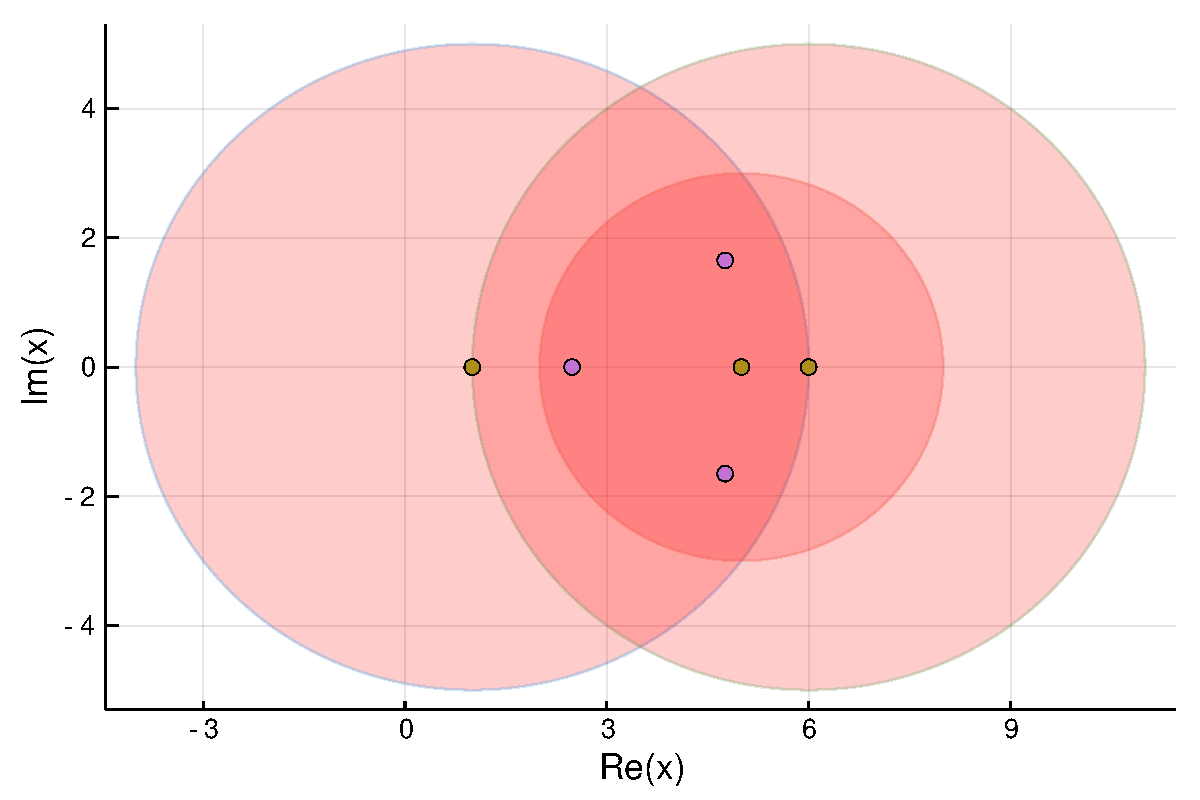
\includegraphics[width=\linewidth]{figures/Lecture8_3_1.pdf}

We can therefore use this to choose a contour big enough to surround all the circles. Here's a fairly simplistic construction for our case where everything is real:


\begin{lstlisting}
(*@\HLJLn{z\ensuremath{\_0}}@*) (*@\HLJLoB{=}@*) (*@\HLJLp{(}@*)(*@\HLJLnf{maximum}@*)(*@\HLJLp{(}@*)(*@\HLJLnf{diag}@*)(*@\HLJLp{(}@*)(*@\HLJLn{A}@*)(*@\HLJLp{)}@*) (*@\HLJLoB{.+}@*) (*@\HLJLn{R}@*)(*@\HLJLp{)}@*) (*@\HLJLoB{+}@*) (*@\HLJLnf{minimum}@*)(*@\HLJLp{(}@*)(*@\HLJLnf{diag}@*)(*@\HLJLp{(}@*)(*@\HLJLn{A}@*)(*@\HLJLp{)}@*) (*@\HLJLoB{.-}@*) (*@\HLJLn{R}@*)(*@\HLJLp{))}@*) (*@\HLJLoB{/}@*)(*@\HLJLni{2}@*) (*@\HLJLcs{{\#}}@*) (*@\HLJLcs{average}@*) (*@\HLJLcs{edges}@*) (*@\HLJLcs{of}@*) (*@\HLJLcs{circle}@*)
(*@\HLJLn{r}@*) (*@\HLJLoB{=}@*) (*@\HLJLnf{max}@*)(*@\HLJLp{(}@*)(*@\HLJLn{abs}@*)(*@\HLJLoB{.}@*)(*@\HLJLp{(}@*)(*@\HLJLnf{diag}@*)(*@\HLJLp{(}@*)(*@\HLJLn{A}@*)(*@\HLJLp{)}@*) (*@\HLJLoB{.-}@*) (*@\HLJLn{R}@*) (*@\HLJLoB{.-}@*) (*@\HLJLn{z\ensuremath{\_0}}@*)(*@\HLJLp{)}@*)(*@\HLJLoB{...}@*)(*@\HLJLp{,}@*) (*@\HLJLn{abs}@*)(*@\HLJLoB{.}@*)(*@\HLJLp{(}@*)(*@\HLJLnf{diag}@*)(*@\HLJLp{(}@*)(*@\HLJLn{A}@*)(*@\HLJLp{)}@*) (*@\HLJLoB{.+}@*) (*@\HLJLn{R}@*) (*@\HLJLoB{.-}@*) (*@\HLJLn{z\ensuremath{\_0}}@*)(*@\HLJLp{)}@*)(*@\HLJLoB{...}@*)(*@\HLJLp{)}@*)

(*@\HLJLnf{plot!}@*)(*@\HLJLp{(}@*)(*@\HLJLnf{Circle}@*)(*@\HLJLp{(}@*)(*@\HLJLn{z\ensuremath{\_0}}@*)(*@\HLJLp{,}@*) (*@\HLJLn{r}@*)(*@\HLJLp{))}@*)
\end{lstlisting}

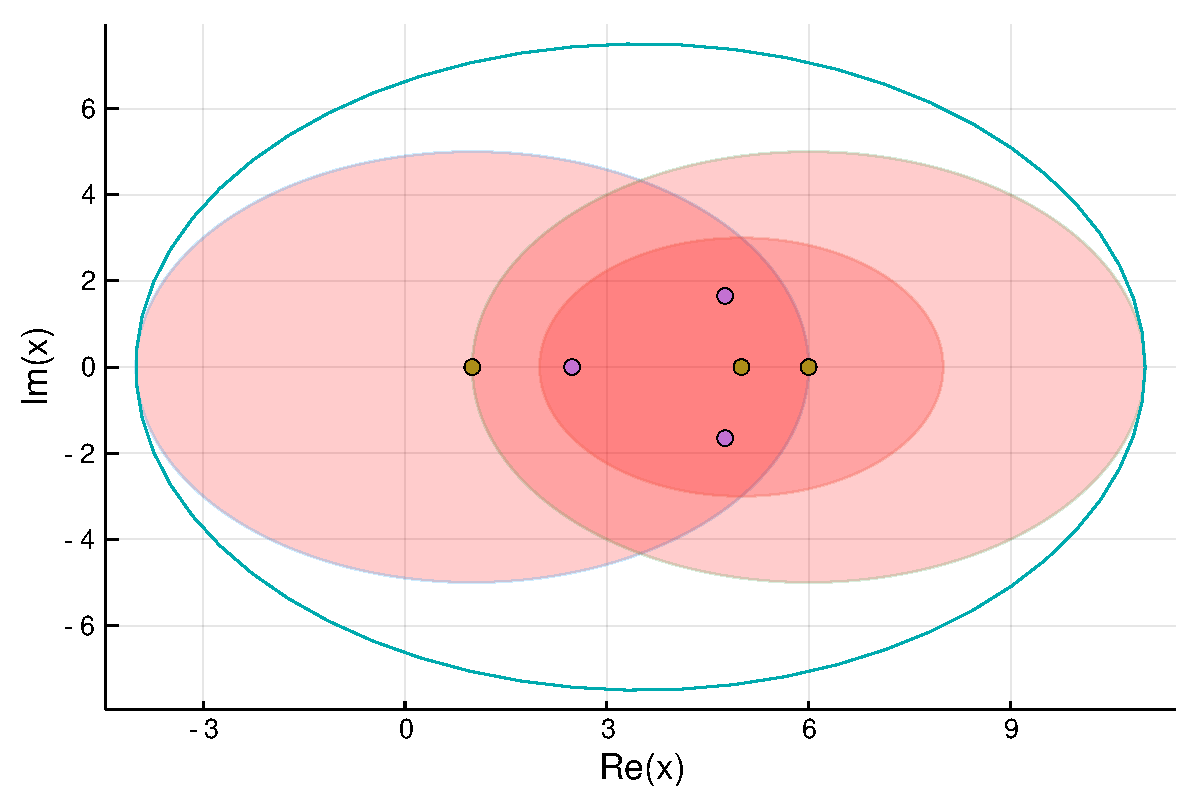
\includegraphics[width=\linewidth]{figures/Lecture8_4_1.pdf}


\end{document}
